\documentclass{beamer}
\usepackage{amsmath}
\usepackage[english]{babel} %set language; note: after changing this, you need to delete all auxiliary files to recompile
\usepackage[utf8]{inputenc} %define file encoding; latin1 is the other often used option
\usepackage{csquotes} % provides context sensitive quotation facilities
\usepackage{graphicx} %allows for inserting figures
\usepackage{booktabs} % for table formatting without vertical lines
\usepackage{textcomp} % allow for example using the Euro sign with \texteuro
\usepackage{stackengine}
\usepackage{wasysym}
\usepackage{tikzsymbols}
\usepackage{textcomp}
% ELIMINAR COMANDOS DE NAVEGACION%%%%%%%%%%%
\setbeamertemplate{navigation symbols}

%\newcommand{\bubblethis}[2]{
 %       \tikz[remember picture,baseline]{\node[anchor=base,inner sep=0,outer sep=0]%
 %       (#1) {\underline{#1}};\node[overlay,cloud callout,callout relative pointer={(0.2cm,-0.7cm)},%
 %       aspect=2.5,fill=yellow!90] at ($(#1.north)+(-0.5cm,1.6cm)$) {#2};}%
 %   }%
%\tikzset{face/.style={shape=circle,minimum size=4ex,shading=radial,outer sep=0pt,
 %       inner color=white!50!yellow,outer color= yellow!70!orange}}

%% Some commands to make the code easier
\newcommand{\emoticon}[1][]{%
  \node[face,#1] (emoticon) {};
  %% The eyes are fixed.
  \draw[fill=white] (-1ex,0ex) ..controls (-0.5ex,0.2ex)and(0.5ex,0.2ex)..
        (1ex,0.0ex) ..controls ( 1.5ex,1.5ex)and( 0.2ex,1.7ex)..
        (0ex,0.4ex) ..controls (-0.2ex,1.7ex)and(-1.5ex,1.5ex)..
        (-1ex,0ex)--cycle;}
\newcommand{\pupils}{
  %% standard pupils
  \fill[shift={(0.5ex,0.5ex)},rotate=80] 
       (0,0) ellipse (0.3ex and 0.15ex);
  \fill[shift={(-0.5ex,0.5ex)},rotate=100] 
       (0,0) ellipse (0.3ex and 0.15ex);}

\newcommand{\emoticonname}[1]{
  \node[below=1ex of emoticon,font=\footnotesize,
        minimum width=4cm]{#1};}
\usepackage{scalerel}
\usetikzlibrary{positioning}
\usepackage{xcolor,amssymb}
\newcommand\dangersignb[1][2ex]{%
  \scaleto{\stackengine{0.3pt}{\scalebox{1.1}[.9]{%
  \color{red}$\blacktriangle$}}{\tiny\bfseries !}{O}{c}{F}{F}{L}}{#1}%
}
\newcommand\dangersignw[1][2ex]{%
  \scaleto{\stackengine{0.3pt}{\scalebox{1.1}[.9]{%
  \color{red}$\blacktriangle$}}{\color{white}\tiny\bfseries !}{O}{c}{F}{F}{L}}{#1}%
}
\usepackage{fontawesome} % Social Icons
\usepackage{epstopdf} % allow embedding eps-figures
\usepackage{tikz} % allows drawing figures
\usepackage{amsmath,amssymb,amsthm} %advanced math facilities
\usepackage{lmodern} %uses font that support italic and bold at the same time
\usepackage{tikz}
\hypersetup{
    colorlinks=true,
    linkcolor=blue,
    filecolor=magenta,      
    urlcolor=blue,
}
\usepackage{tcolorbox}
\usepackage{hyperref}

\usefonttheme[onlymath]{serif} %set math font to serif ones

\definecolor{beamerblue}{rgb}{0.2,0.2,0.7} %define beamerblue color for later use

%%% defines highlight command to set text blue
\newcommand{\highlight}[1]{{\color{blue}{#1}}}


%%%%%%% commands defining backup slides so that frame numbering is correct

\newcommand{\backupbegin}{
   \newcounter{framenumberappendix}
   \setcounter{framenumberappendix}{\value{framenumber}}
}
\newcommand{\backupend}{
   \addtocounter{framenumberappendix}{-\value{framenumber}}
   \addtocounter{framenumber}{\value{framenumberappendix}}
}

%%%% end of defining backup slides

%Specify figure caption, see also http://tex.stackexchange.com/questions/155738/caption-package-not-working-with-beamer
\setbeamertemplate{caption}{\insertcaption} %redefines caption to remove label "Figure".
%\setbeamerfont{caption}{size=\scriptsize,shape=\itshape,series=\bfseries} %sets figure  caption bold and italic and makes it smaller


\usetheme{Boadilla}

%set options of hyperref package
\hypersetup{
    bookmarksnumbered=true, %put section numbers in bookmarks
    naturalnames=true, %use LATEX-computed names for links
    citebordercolor={1 1 1}, %color of border around cites, here: white, i.e. invisible
    linkbordercolor={1 1 1}, %color of border around links, here: white, i.e. invisible
    colorlinks=true, %color links
    anchorcolor=black, %set color of anchors
    linkcolor=beamerblue, %set link color to beamer blue
    citecolor=blue, %set cite color to beamer blue
    pdfpagemode=UseThumbs, %set default mode of PDF display
    breaklinks=true, %break long links
    pdfstartpage=1 %start at first page
    }
% You can copy any following box you like to your code.
\newtcolorbox{boxA}{
    fontupper = \bf,
    boxrule = 1.5pt,
    colframe = black % frame color
}

% --------------------
% Overall information
% --------------------
\title[Principios de Economía]{Principios de Economía \vspace{4mm}
\\ Magistral 2}
\date{}
\author[Riottini]{Franco Riottini}
\vspace{0.4cm}
\institute[]{Universidad de San Andrés} 

\begin{document}

\begin{frame}
\titlepage
\centering

\includegraphics[scale=0.2]{../Figures/logoUDESA.jpg} 
\end{frame}


\begin{frame}
\frametitle{La economía, los modelos y las funciones}
\begin{itemize}
    \item La economía estudia cómo asignar recursos escasos de forma eficiente, y \vspace{2mm}
    \item Recordemos que las funciones (y sus expresiones matemáticas y gráficas) nos ayudan a representar ideas... \vspace{2mm}
    \item Vamos a utilizar funciones para crear un modelo que nos permita analizar como los individuos manejan la ESCASEZ 
    \begin{itemize}
        \item ¿Qué significa que los recursos son escasos? ¡Que no hay de todo para todos! 
    \end{itemize}
    \item Inmediatamente aparece otro concepto importante: las personas enfrentan trade-offs
\end{itemize} 
\end{frame}

\begin{frame}
\frametitle{Escasez}
\begin{itemize}
    \item Tomar una decisión implica tener más de una alternativa \vspace{2mm}
    \item Pero los recursos son escasos...  
    \item El problema surge porque las necesidades humanas son, en la práctica, ilimitadas, mientras que los recursos económicos son limitados. 
    \item Entonces, la escasez representa básicamente una restricción o límite que nos obliga a elegir entre alternativas.
    \vspace{2mm}
\end{itemize} 
\end{frame}

\begin{frame}
\frametitle{Trade-off}
\begin{itemize}
    \item Cada vez que tomamos una decisión y elegimos algo ganamos algo pero también perdemos algo \vspace{2mm}
    \item ¿Cómo tomamos una decisión? 
    \begin{itemize}
        \item Evaluamos todos los beneficios que se obtienen por tomar la decisión y compararlos con todos los costos que resultan de la decisión
        \vspace{1mm}
    \end{itemize}
    \item A veces es fácil pensar en esto, pero otras veces no tanto...
\end{itemize} 
\end{frame}

\begin{frame}
\frametitle{Beneficios y costos}
\begin{itemize}
    \item Beneficios: La cantidad monetaria máxima que estaríamos dispuesto a pagar por hacer X. \vspace{2mm}
    \item Costo: Valor de todos los recursos que resigno para llevar a cabo una actividad X (Sea invertir, estudiar, trabajar, ocio, etc.), en términos monetarios.  \vspace{2mm}
    \item ¿Cómo podemos cuantificar los beneficios y los costos? 
    \begin{itemize}
    \item Cuando disponemos de "precios de mercado" se facilita la cuestión
    \item Veamos ejemplos: Cita o noche de amigos/as; Cambiar una canción.
    
    \end{itemize}
\end{itemize} 
\end{frame}

\begin{frame}
\frametitle{¿Cuáles son los costos relevantes...? }
\begin{itemize}
    \item  \href{https://econ.video/2017/08/28/the-simpsons-opportunity-cost-of-lines/}{El costo de oportunidad}
    \begin{itemize}
        \item El costo de oportunidad de una decisión es el valor al que se renuncia al rechazar la mejor alternativa posible.
    \end{itemize}
    \vspace{2mm}
    \item \textbf{La falacia del costo hundido}  
    \begin{itemize}
        \item Ocurre cuando se están considerando costos y beneficios que no varían con las consecuencias de su decisión
        \item Si voy a tener que afrontar igual un costo sea cual sea la decisión que tome entonces no lo debo tener en cuenta!
    \end{itemize}
    \vspace{2mm}
    \item \href{https://www.goodfood.com.au/eat-out/good-food-guides/the-surprising-costs-of-running-a-restaurant-20180327-h0y23c}{Los costos escondidos} 
    \vspace{2mm}
\end{itemize}
Este forma de pensar nos permite escribir la siguiente regla:
\begin{boxA}
    Elegir una alternativa dada si y sólo si la variación que experimentarán los beneficios como consecuencia de elegir dicha alternativa excede a la variación que experimentarán los costos 
\end{boxA}

\end{frame}

\begin{frame}
\frametitle{Entonces.. }
    \begin{boxA}
        En lo que siempre vamos a estar pensando a lo largo de la materia es en costos marginales y beneficios marginales    
    \end{boxA}
\end{frame}
\begin{frame}
\frametitle{Pensemos algunos casos}
\begin{itemize}
    \item Vamos a usar los conceptos y el modelo para comprender como las personas toman decisiones: \vspace{2mm}
    \begin{itemize} 
    \item ¿Que sucede si \textbf{pierdo} la entrada que compre para el recital de Taylor Swift? \vspace{2mm}
    \item ¿Por qué solo en las grandes ciudades los Remis/Taxis están pintados de un mismo color? \vspace{2mm}
    \item ¿Por qué los colectivos escolares no tienen cinturón de seguridad? 
    \end{itemize}
\end{itemize} 
\end{frame}

\begin{frame}
\frametitle{¿Tik tok es gratis?}
\begin{itemize}
    \item Los Argentinos pasamos en promedio 30 minutos diarios en Tik Tok. \vspace{2mm}
    \item En jóvenes el tiempo puede superar las dos horas diarias. \vspace{2mm}
    \begin{itemize}
    \item ¿Cuál es el costo de oportunidad por hora? \vspace{2mm}
    \item Estimemos el costo de oportunidad total...
    \end{itemize}
\end{itemize} 
\end{frame}

\begin{frame}
\frametitle{La decisión de consumo}
\centering

\includegraphics[scale=0.7]{../Figures/Tema_02.1_pizzabirra.jpg}
\begin{itemize}
\item ¿Qué tiene en cuenta un consumidor al momento de consumir un producto?
\end{itemize}
\end{frame}

\begin{frame}
\frametitle{¿Que información necesitamos?}
\begin{itemize}
\item Necesitamos conocer....
\begin{itemize}
    \item Ingreso/dinero disponible \vspace{2mm}
    \item Precios de todos los productos \vspace{2mm}
    \item Preferencias o gustos
    \end{itemize}
\end{itemize}
\end{frame}

\begin{frame}
\frametitle{El problema del estudiante}
\centering
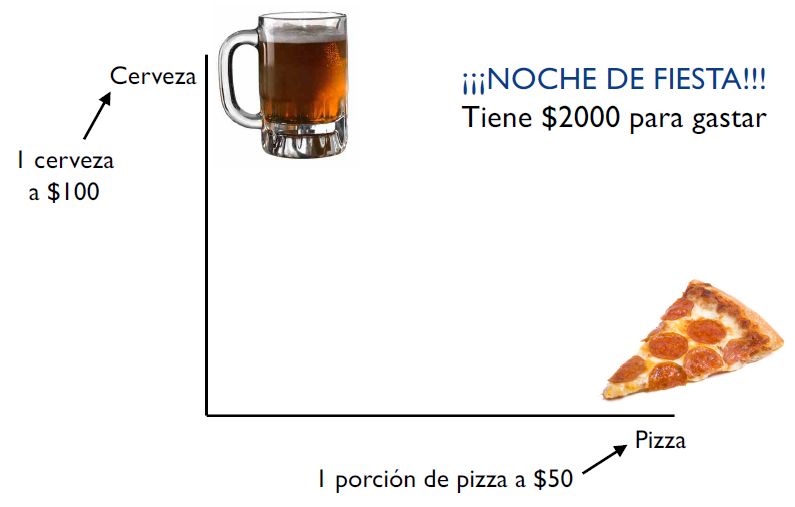
\includegraphics[scale=0.5]{../Figures/Tema_02.2_rp.png}
\end{frame}

\begin{frame}
\frametitle{El problema del estudiante}
\centering
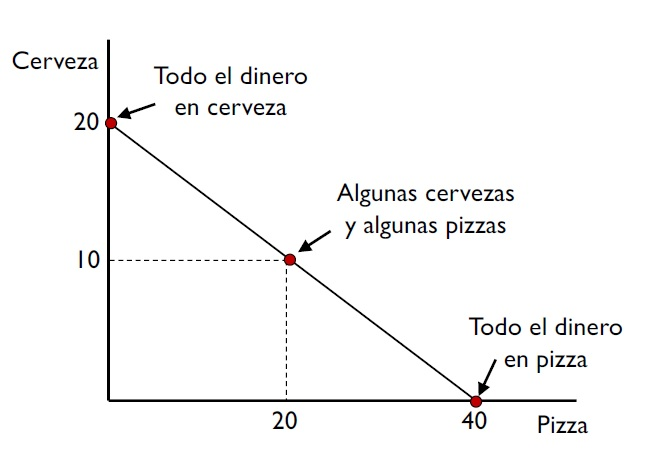
\includegraphics[scale=0.6]{../Figures/Tema_02.3_rp1.jpg}
\end{frame}

\begin{frame}
\frametitle{Restricción presupuestaria}
\centering
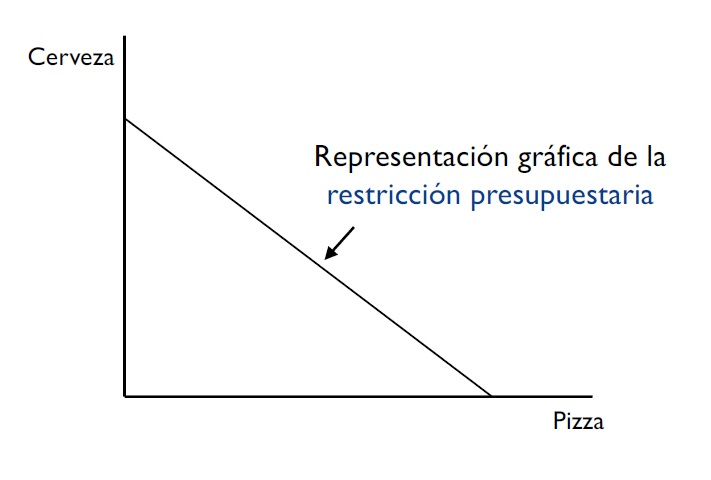
\includegraphics[scale=0.6]{../Figures/Tema_02.4_rp2.jpg}
\end{frame}

\begin{frame}
\frametitle{¿Cuánto puede consumir?}
\centering
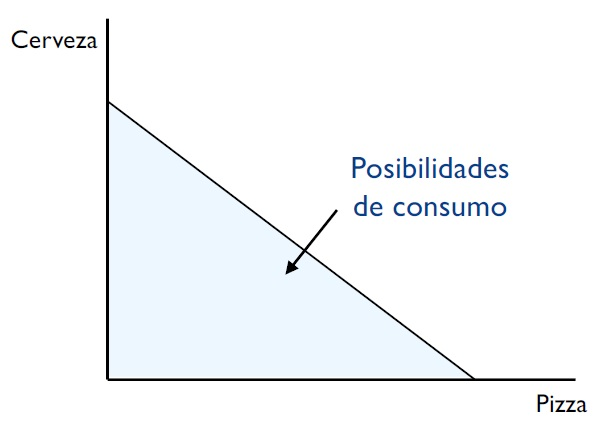
\includegraphics[scale=0.6]{../Figures/Tema_02.5_rp3.jpg}
\end{frame}

\begin{frame}
\frametitle{El precio de la pizza}
\centering
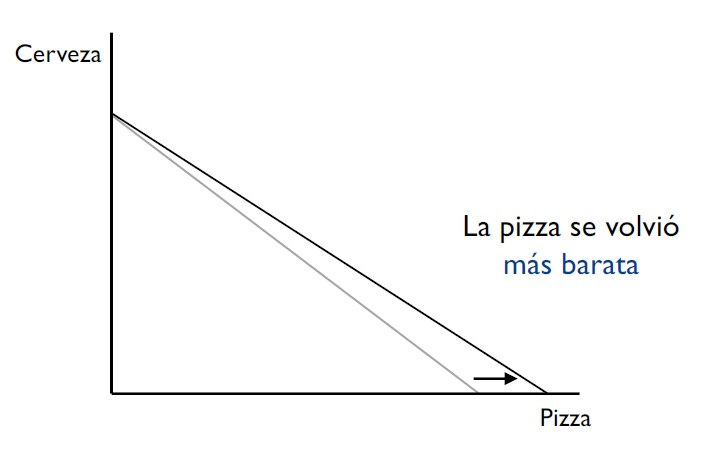
\includegraphics[scale=0.6]{../Figures/Tema_02.6_rp4.jpg}
\end{frame}

\begin{frame}
\frametitle{El precio de la cerveza}
\centering
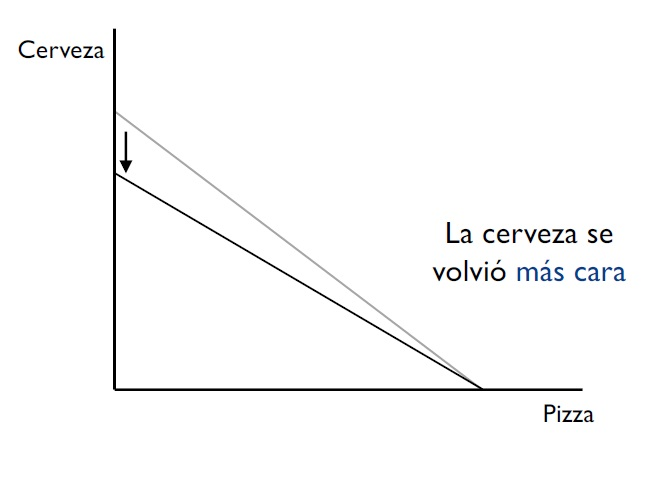
\includegraphics[scale=0.6]{../Figures/Tema_02.7_rp5.jpg}
\end{frame}

\begin{frame}
\frametitle{Precios relativos}
\centering
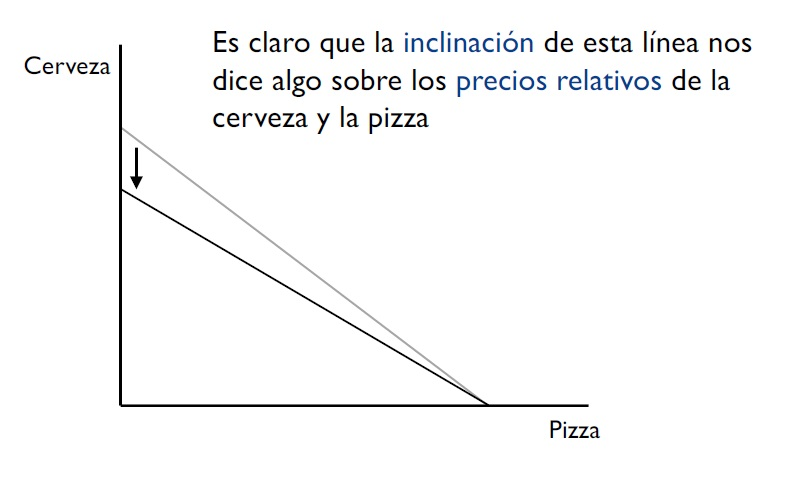
\includegraphics[scale=0.55]{../Figures/Tema_02.8_rp6.jpg}
\end{frame}

\begin{frame}
\frametitle{Pendiente}
\begin{itemize}
    \item Llamamos "pendiente" a la inclinación de una función en un punto particular.
    \item En general, va a estar determinada por el cambio vertical con respecto al cambio horizontal. \\ \vspace{2mm}
    \begin{center}
        $Pendiente =\frac{\Delta Y}{\Delta X} = \frac{\text{Cambio Vertical}}
    {\text{Cambio Horizontal}}$
    \end{center}
\end{itemize} 
Ahora bien, si nos movemos a lo largo de la restricción presupuestaria, se va a cumplir que lo que dejo de gastar en un bien tiene que ser igual a lo que comienzo a gastar del otro. Por ende:
\begin{center}
    \[-\Delta Y \times P_Y = \Delta X \times P_X \]
\end{center}
Reordenando esa ecuación, obtenemos que:
\begin{center}
    \[\frac{\Delta Y}{\Delta X} = -\frac{P_X}{P_Y} \]
\end{center}
Que es lo mismo que la pendiente!

\end{frame}

\begin{frame}
\frametitle{Pendiente}
    \begin{itemize}
        \item En el caso de la restricción presupuestaria del ejemplo \\
        \begin{center}
            $Pendiente = - \frac{\text{Precio Pizza}}{\text{Precio Cerveza}}= -\frac{P_P}{P_C} = -\frac{50}{100} = -\frac{1}{2}$
        \end{center}
        \item Esto nos da una noción de cuanto debo resignar de un bien para poder consumir una unidad más del otro.
        \item En este caso, me dice que si resigno una pizza puedo consumir media cerveza más.
    \end{itemize}
\end{frame}

\begin{frame}
\frametitle{Tasa Marginal de Transformación}
\begin{itemize}
    \item La Tasa Marginal de Transformación (TMT) es la cantidad de un bien que el consumidor debe renunciar para obtener una unidad más del otro bien.
    \item Viene determinado por los precios de los bienes en el mercado.\\ \vspace{6mm} 
    \begin{center}
      $TMT = - \frac{\text{Precio Pizza}}{\text{Precio Cerveza}}$
      \end{center}
\end{itemize} 
\end{frame}

\begin{frame}
\frametitle{Si rompemos el chanchito o vamos a la casa de la abuela...}
\centering
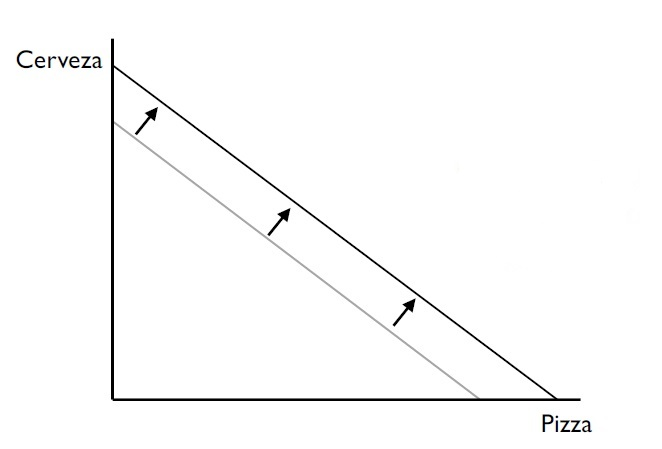
\includegraphics[scale=0.55]{../Figures/Tema_02.9_rp7.jpg}
\end{frame}

\begin{frame}
\frametitle{Recursos}
\centering
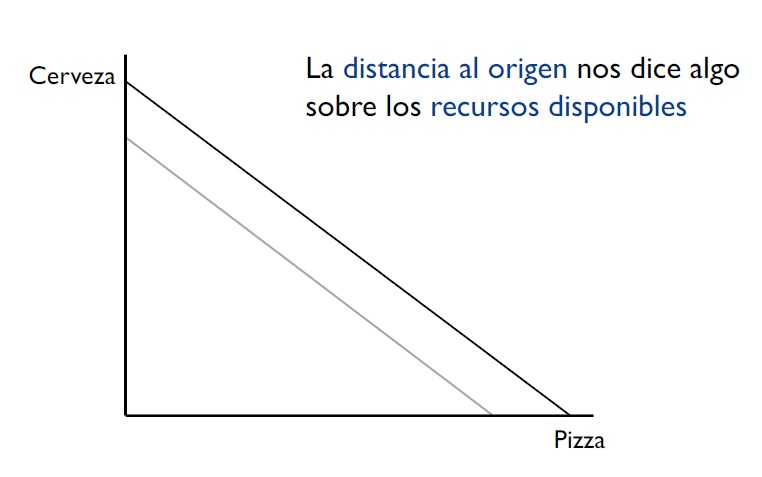
\includegraphics[scale=0.55]{../Figures/Tema_02.10_rp8.jpg}
\end{frame}

\begin{frame}
\frametitle{Restricción presupuestaria}
\begin{itemize}
    \item La representación gráfica de la restricción presupuestaria es útil para ver:
    \begin{itemize}
        \item Posibilidades de consumo
        \item Precios relativos de los bienes
    \end{itemize}
    \item Pero lo mismo se puede ver estudiando la expresión matemática \\ \vspace{2mm}
    \begin{center}
    $Ingresos$ = $P_{Cerveza} * Q_{Cerveza}$ + $P_{Pizza} * Q_{Pizza}$
    \\
    \end{center}\vspace{2mm}
    \item De hecho, las expresiones matemáticas pueden ser mas flexibles que las representaciones gráficas...
    \item Los economistas usan mucho ambas (junto con palabras), para construir modelos.
\end{itemize} 
\end{frame}

\begin{frame}
\frametitle{Algunos casos especiales}
\begin{itemize}
\item En los casos analizados asumimos que el precio del producto no cambia según la cantidad de unidades que adquirimos
\item En muchos casos no es así...
\end{itemize}
\vspace{3mm}
\centering

\includegraphics[scale=0.55]{../Figures/Lentes.jpeg}
\end{frame}


\end{document}
